\section{Evaluation}
\subsection{Participants}
Fifteen subjects (5 female) participated in the study.
Each subject took about 30 minutes to complete the study.

\subsection{Phrase Set}
We selected fifty phrases from a collection of five-hundred phrases commonly used for text entry evaluations~\cite{mackenzie2003phrase}.
To allow for cross-comparison to other text entry methods, the corpus doesn't include phrases with punctuation marks.
Non-alphanumeric symbols are rarely considered in text input research~\cite{mackenzie2003phrase} even though some punctuations (. - ' ( ) ") are more frequent than the least common English letter (q)~\cite{malikpunctuation}.
 
SwipeVR allows for the entry of non-alphanumeric symbols using a different interaction technique for words then for punctuation and characters.
To measure the  we add to the phrase set ten phrases for the user to enter that contain non-alphanumeric symbols.
We add five phrases with punctuation marks so the evaluation more closely mimics real-life interactions.
This addition more fully tests the transition time between interaction techniques. 

Copying pre-selected phrase is usually the preferred method for text entry when doing evaluations in a lab setting~\cite{mackenzie2002character, mackenzie2003phrase}.
Although, copying pre-selected entry rates should be regarded differently from true, ``in the wild'' results when the user is composing text instead of transcribing prompted phrases.
In particular, reading a pre-selected phrase has a noticalbly different cadence and certainty that is typically not present in natural voice interactions which leads to what we hypothesize could be an optimistic measurement of voice input.

When the user composes text on their own, there could be substantial thinking time ~\cite{shneiderman2000limits} and other considerations that are difficult to measure.
We only use pre-selected phrases and rely on qualitative feedback to develop a holistic understanding for usability.

\subsection{Procedure}
Participants entered a series of phrases from the phrase set.
One of our metrics is the learnability of the system so we don't give users practice trials before beginning the actual test.

For each user we conduct twelve sequential sessions.
In each session, a user enters six phrases.
After entering all the phrases with both input methods, the participant filled out
a questionnaire regarding their quantitative feedback on the text entry method.
Finally, subjects were asked for additional comments.

\subsection{Measures}
In the field of text entry, several metrics are used to characterize a method's performance ~\cite{wobbrock2007measures,arif2009analysis}.
Here, we discuss the performance metrics we use to evaluate the performance of the input device.  

\subsubsection{Words per Minute}
Words per minute (~$WPM$) is perhaps the most widely reported empirical measure of
text entry performance~\cite{wobbrock2007measures}:

\[ 
WPM={\vert T\vert -1\over S}\times 60\times{1\over 5}. \eqno{\hbox{(1)}}
\]

Where, $S$ is the time in seconds from the first key press to the last, which means that the entry of the first character is never timed, which is the motivation for the "- 1" in the numerator of (1)~\cite{yamada1980historical}.
English words by convention are treated as having five characters~\cite{yamada1980historical}.

\subsubsection{Error Rate}
Error Rate (~$ER$) is the ratio of the total number of incorrect characters in the transcribed text to the length of the transcribed text:

\[
ER={INF\over \vert T\vert }\times 100\%. \eqno{\hbox{(2)}}
\]

Where, Incorrect Not Fixed (~$INF$) is the number of unnoticed incorrect characters in the transcribed text.


\begin{table}\centering
\ra{1.3}
\begin{tabular}{@{}rrrrr@{}}\toprule
            &             & $SwipeVR$  \\
\midrule
$Positioning$     &             & relative        \\

%    Correction Method    & X       & X       & X       &   \checkmark    \\ 

\bottomrule
\end{tabular}
\caption{Ontology of input methods.}
\label{table:usability}
\end{table}


\subsubsection{Subjective }
we ask the user to evaluate each entry mechanism on a 5-point Likert Scale (Strongly Disagree, Disagree, neutral, Agree, Strongly Agree).
Additionally, users are  interviewed to further understand the their qualitative experience.

\subsubsection{Performance}
The input device felt responsive\\
The visuals were smooth and didn't freeze\\
The input device worked properly\\
The system was over responsive and showed inputs that I didn't enter\\
The system was under responsive and didn't showed inputs that I thought I entered

\subsubsection{Design}
It is easy to understand what to do with the input device\\
It was easy to learn how to use the input device\\
The interface was intuitive\\
This application has a graphical interface pleasant and understandable\\
The text and input were clearly visible

\subsubsection{Ergonomics}
I felt arm strain\\
I felt hand strain\\
I felt hand Nausea\\
I felt dizzy when using the system\\
I felt nauseous when using the system

\subsubsection{Applications}
I would use the input device to do a web search\\
I would use the input device to write an email\\
I would use the input device in public\\
I would use the input device at home\\
I would use the input device at a park\\
I would use the input device to chat (text)\\
I would use the input device to edit a letter

\section{Results}
\subsection{Word Per Minute}
The average rate for text entry was 34 WPM.  

\subsection{Error Rate}
The average error rate for text entry was 4\%.  

\begin{figure}
\centering

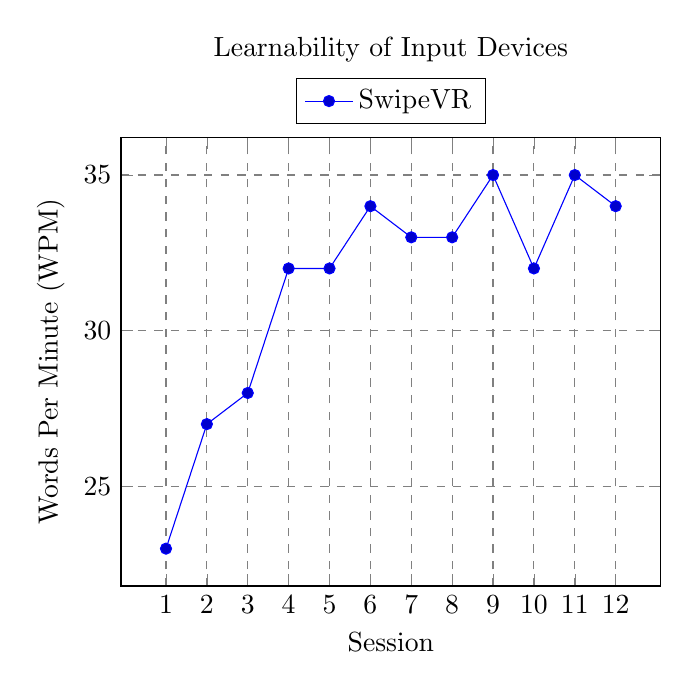
\begin{tikzpicture}
\pgfplotsset{
    every axis legend/.append style={
      at={(0.5,1.03)
    },
    anchor=south
    }
}
\pgfplotsset{grid style={dashed,gray}}
%\pgfplotsset{minor grid style={dashed,red}}
%\pgfplotsset{major grid style={dotted,green!50!black}}

\begin{axis}[
legend columns=-1,
xlabel=Session,
ylabel=Words Per Minute (WPM),
 title style={at={(0.5,0)},anchor=south,yshift=180},
 title = Learnability of Input Devices,
 %ytick={0,5,10,15,20},
 %minor ytick={1,2,3,4,5,6,7,8,9,10,11,12,13,14,15,16,17,18,19,20},
 xtick={1,2,3,4,5,6,7,8,9,10,11,12},
 %minor xtick={1,2,3,4,5,6,7,8,9,10,11,12,13,14,15,16,17,18,19,20},
 grid=both,
]
\addplot coordinates
{
  (1,23)(2,27)(3,28)(4,32)(5,32)(6,34)(7,33)(8,33)(9,35)(10,32)(11,35)(12,34)
};

\legend{SwipeVR, Speech, Gaze, Mobile}

\end{axis}
\end{tikzpicture}

%4.7.1 Markers for graph fixing the circle, square, x, triangle overloading

\caption{
Graph of learnability for each of the input methods.
Learning curves for the four tested entry methods.
Entry rate on each block of 20 sentences in the second pilot.
Each line is a single participant.
}~\label{fig:learnability}
\end{figure}


\subsection{Learnability}
The extrapolated learning curve is shown in Figure~\ref{fig:learnability}.
A curve is fit according to a power law and allow us to speculate about performance in future sessions.

\subsection{Usability}
We found that the 

\begin{figure}
\centering
  \begin{tikzpicture}[scale=.6]

      \pie{44/Word entry with thumb not on trackpad, 3/Thumb on trackpad, 29/Between word, 24/Editing}[explode=0.1]
  \end{tikzpicture}
  \caption{The majority of time the user was entering a word, their thumb was not on the trackpad.  There was also a delay between when the user was entering words.
    }
  ~\label{fig:distance}
  \end{figure}

\begin{figure}
\centering
\includegraphics[width=0.5\columnwidth]{figures/circle}
  \caption{Sample of a right-handed users's swipes.  Most of the swipes are concetrated in the upper-left quadrant of the circluar trackpad.}

\label{fig:circle}

\end{figure}

\begin{figure}
\centering
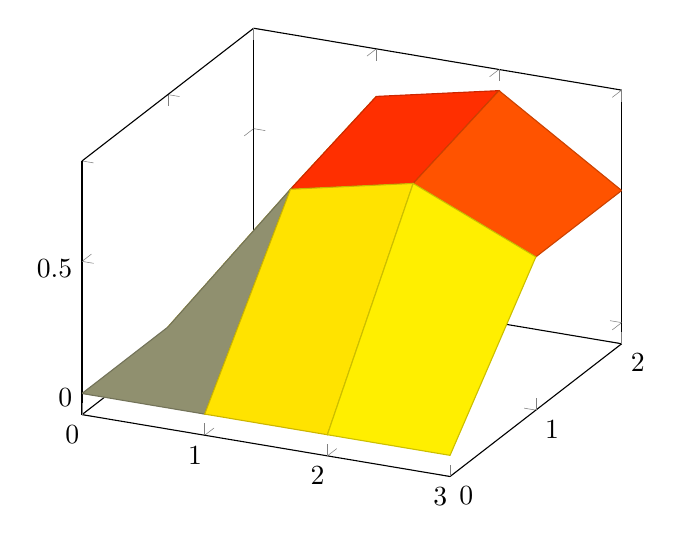
\begin{tikzpicture}
\begin{axis}
% this yields also a 3x4 matrix:
\addplot3[surf,mesh/rows=3] coordinates {
(0,0,0) (1,0,0) (2,0,0) (3,0,0)
(0,1,0) (1,1,0.6) (2,1,0.7) (3,1,0.5)
(0,2,0) (1,2,0.7) (2,2,0.8) (3,2,0.5)
};
\end{axis}
\end{tikzpicture}


  \caption{(Bar graph of arm strain, hand strain, neck strain, dizziness/nausea)  Differences between the initial and final subjective comfort ratings for each of the four techniques in the experiment 
}~\label{fig:graphLearning}
\end{figure}

\begin{figure}
\centering

  \includegraphics[width=0.9\columnwidth]{figures/sigchi-logo}

  \caption{(Participants' subjective evaluation of difficulty 
}~\label{fig:graphLikert}
\end{figure}

\section{Discussion}
We argue that we have confirmed H1, H2, and H3.

Concerning H1 (SwipeVR faster than gaze), we find there are significant differences between text entry rates of both approaches.

